\documentclass[tikz]{standalone}
\usepackage{pgfplots}
\pgfplotsset{compat=newest}
\pgfplotsset{every axis legend/.append style={%
cells={anchor=west}}
}
\usepgfplotslibrary{polar}
\usetikzlibrary{arrows}
\tikzset{>=stealth'}

\begin{document}
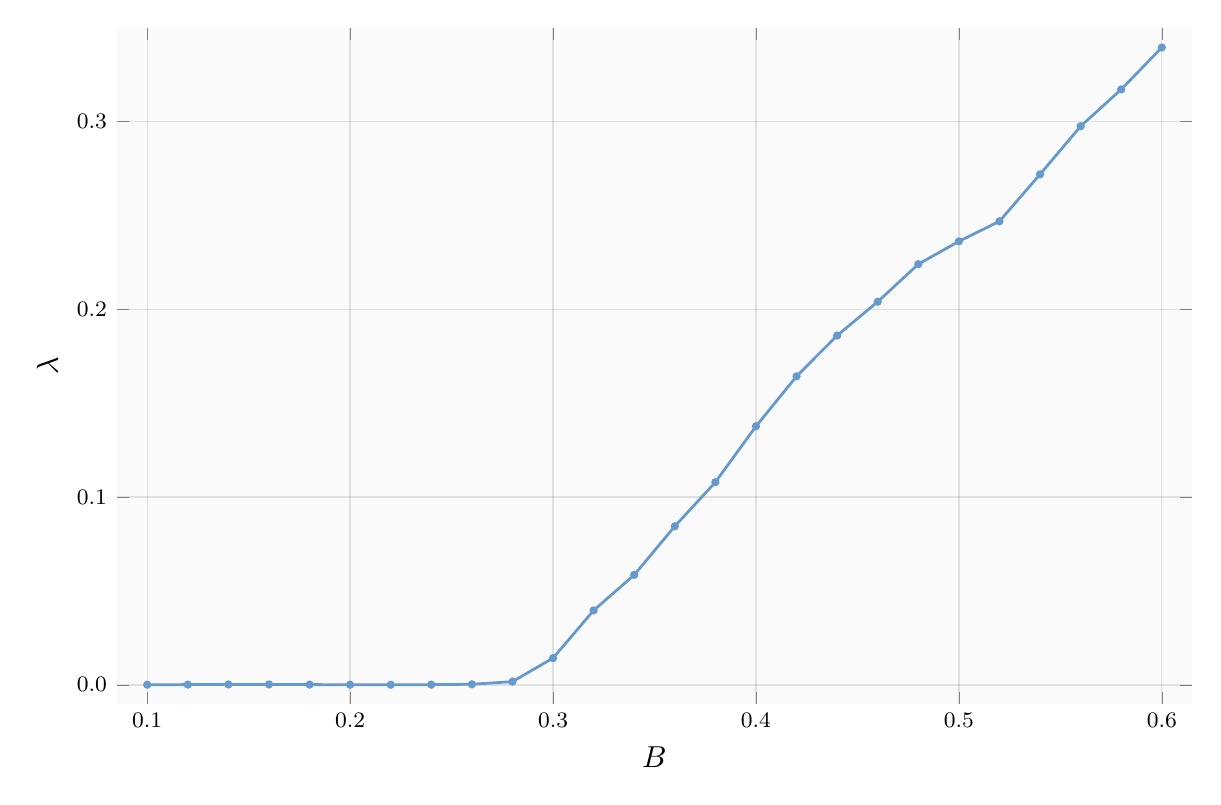
\begin{tikzpicture}[]
\begin{axis}[height = {101.6mm}, ylabel = {$\lambda$}, xmin = {0.085}, xmax = {0.615}, ymax = {0.349666918987477}, xlabel = {$B$}, unbounded coords=jump,scaled x ticks = false,xlabel style = {font = {\fontsize{11 pt}{14.3 pt}\selectfont}, color = {rgb,1:red,0.00000000;green,0.00000000;blue,0.00000000}, draw opacity = 1.0, rotate = 0.0},xmajorgrids = true,xtick = {0.1,0.2,0.30000000000000004,0.4,0.5,0.6000000000000001},xticklabels = {$0.1$,$0.2$,$0.3$,$0.4$,$0.5$,$0.6$},xtick align = inside,xticklabel style = {font = {\fontsize{8 pt}{10.4 pt}\selectfont}, color = {rgb,1:red,0.00000000;green,0.00000000;blue,0.00000000}, draw opacity = 1.0, rotate = 0.0},x grid style = {color = {rgb,1:red,0.00000000;green,0.00000000;blue,0.00000000},
draw opacity = 0.1,
line width = 0.5,
solid},x axis line style = {draw opacity = 0},scaled y ticks = false,ylabel style = {font = {\fontsize{11 pt}{14.3 pt}\selectfont}, color = {rgb,1:red,0.00000000;green,0.00000000;blue,0.00000000}, draw opacity = 1.0, rotate = 0.0},ymajorgrids = true,ytick = {0.0,0.1,0.2,0.30000000000000004},yticklabels = {$0.0$,$0.1$,$0.2$,$0.3$},ytick align = inside,yticklabel style = {font = {\fontsize{8 pt}{10.4 pt}\selectfont}, color = {rgb,1:red,0.00000000;green,0.00000000;blue,0.00000000}, draw opacity = 1.0, rotate = 0.0},y grid style = {color = {rgb,1:red,0.00000000;green,0.00000000;blue,0.00000000},
draw opacity = 0.1,
line width = 0.5,
solid},y axis line style = {draw opacity = 0},    xshift = 0.0mm,
    yshift = 0.0mm,
    axis background/.style={fill={rgb,1:red,0.98039216;green,0.98039216;blue,0.98039216}}
,legend style = {color = {rgb,1:red,0.00000000;green,0.00000000;blue,0.00000000},
draw opacity = 1.0,
line width = 1,
solid,fill = {rgb,1:red,0.98039216;green,0.98039216;blue,0.98039216},font = {\fontsize{8 pt}{10.4 pt}\selectfont}},colorbar style={title=}, ymin = {-0.010135019217953156}, width = {152.4mm}]\addplot+ [color = {rgb,1:red,0.40000000;green,0.60000000;blue,0.80000000},
draw opacity = 1.0,
line width = 1,
solid,mark = *,
mark size = 1.5,
mark options = {
    color = {rgb,1:red,0.00000000;green,0.00000000;blue,0.00000000}, draw opacity = 0.0,
    fill = {rgb,1:red,0.40000000;green,0.60000000;blue,0.80000000}, fill opacity = 1.0,
    line width = 0,
    rotate = 0,
    solid
},forget plot]coordinates {
(0.1, 5.708376965712037e-5)
(0.12, 0.00010104874943593509)
(0.14, 0.0001786436263554426)
(0.16, 0.00019647650964605383)
(0.18, 0.00011131058110963566)
(0.2, 4.997112106467777e-5)
(0.22, 4.805450484203611e-5)
(0.24, 8.483267811896845e-5)
(0.26, 0.00029511328493953107)
(0.28, 0.0016862210175077072)
(0.3, 0.01425075227612393)
(0.32, 0.039614780352864455)
(0.34, 0.05853422780733186)
(0.36, 0.0844481684554568)
(0.38, 0.10792961000313718)
(0.4, 0.13771347684280638)
(0.42, 0.1643039642486243)
(0.44, 0.18604819882971585)
(0.46, 0.20404591397616814)
(0.48, 0.22405520921604624)
(0.5, 0.23621254731659908)
(0.52, 0.24689641636431545)
(0.54, 0.27191532958449716)
(0.56, 0.2975246781898004)
(0.58, 0.3171463970050902)
(0.6, 0.3394838452646818)
};
\end{axis}

\end{tikzpicture}
\end{document}
